Machine learning is a sub-field of \gls{AI} within the broad category of
computer science. The goal of \gls{AI} is to create computer systems that
respond to their environment according to some set of criteria or goal. For
example, self-driving vehicles have computers on board that learn to avoid
curbs and humans. It is common knowledge that the use of \gls{AI} has been
expanding at a rapid rate in recent years. News stories of major tech
companies' \gls{AI} advancements are frequent and news articles abound with
data on which jobs will be replaced with \gls{AI} in the near future. 

While its use has been increasing in the commercial sector, there is also much
anecdotal evidence to support the existence of a rapid increase of \gls{AI} use
in academic research across many disciplines beyond robotics. \gls{AI} systems
have been used in detection (e.g., fraud or spam), medical diagnostics, user
analysis (e.g., Netflix ratings), and a host of scientific disciplines that
have increasing amounts of multivariate data.

Much of the recent advances to the field of \gls{AI} have occured in the
statistical realm, which forgoes domain knowledge in favor of large data sets.
Thus, machine learning and statistical learning has become somewhat of a
separate field. \todo{could explain more, cite changing science of ML} Machine
learning research focuses on the underlying algorithms using mathematical
optimization, methods for pattern recognition, and computational statistics.
As an application, however, this study is not concerned with computational
time, but rather the ability to correctly predict values and categories
relevant to the nuclear forensics mission. This restricts the relevancy of the
algorithms to the underlying theory and its impact on the resulting model's
accuracy. 

Machine learning algorithms can be separated into two main categories:
unsupervised and supervised learning.  The former groups or interprets a set of
input data, predicting patterns or structures. The latter includes both the
input and output data, enabling the trained model to predict future outputs.
Broadly speaking, the unsupervised learning algorithms are designed for
clustering data sets or dimensionality reduction (i.e., determining some subset
or linear combination of features most relevant to the input data) of data
sets.  Supervised learning algorithms predict both discrete and continuous
values via classification and regression, respectively. Some algorithms can
perform both classification and regression, and neural networks can even be
modified to perform either supervised or unsupervised learning. Additionally,
various algorithms can be strung together, which is referred to as \textit{ensemble
methods}. One common way of doing this is performing deimensionality reduction
prior to supervised learning.\todo{check that this common workflow qualifies as
ensemble} 

As shown in Figure \ref{fig:supervised}, a typical (supervised) machine
learning workflow begins with a training data set, which has a number of
\textit{instances}, or rows of observations of .  Each instance has some \textit{attributes}, also referred to as \textit{features}, and a label, which
can be a categorical label or discrete/continuous values.  The training data
are then inserted into a statistical learner; this calculates some objective,
minimizes or maximizes that objective, and provides some model. This model is
typically evaluated using a test set that has the same set of attributes and
labels (but different instances). The comparison of what the model predicts and
the actual label gives the \textit{testing error}. Depending on the performance
and application, the model may need improvement from more training and/or some
changes in the algorithm parameters. Once the model is performing well enough,
it is finalized; then a user can provide a single instance and a value can be
predicted from that. 

\begin{figure}[h!]
  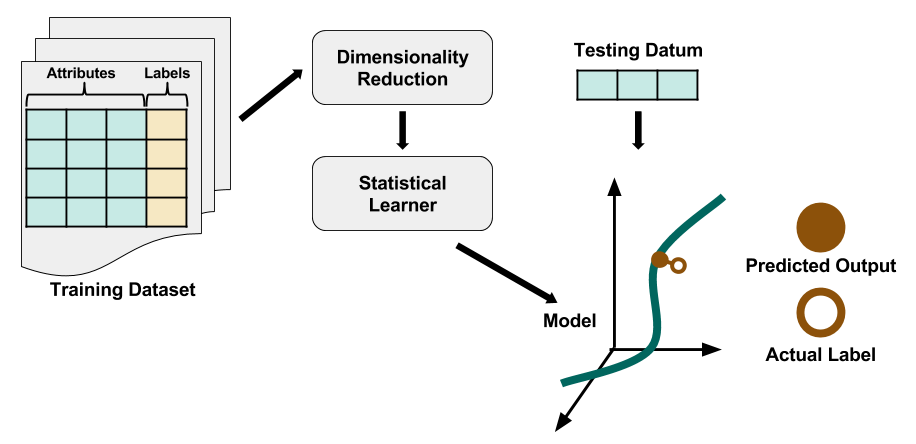
\includegraphics[width=\linewidth]{./chapters/intro/SupervisedRegression.png}
  \caption{Schematic representing the workflow of a statistical learning regression algorithm.}
  \label{fig:supervised}
\end{figure}

This study performs both classification and regression tasks using supervised
learning algorithms.  Differences among the underlying mathematics \todo{phrase
better} of the algorithms do impact the performance of a machine-learned model.
Therefore the algorithms used in this study will be discussed in
Section \ref{sec:algs}. Additionally, evaluating algorithm performance is 
important and will be covered in Section \ref{sec:diagnostics}. Finally, 
robustly comparing different algorithms continues the previous discussion on 
inverse problem theory and is in Section \ref{sec:selection}.

\subsection{Classification and Regression Algorithms}
\label{sec:algs}

For relevant nuclear forensics predictions, both classification and regression
algorithms must be used.  For example, one may want to predict the reactor type
based on some measurements (referred to as features) of spent fuel of an
unknown source, and this would require a classification algorithm. Or perhaps
the input fuel composition is relevant to an investigation on weapons intent,
so a regression algorithm would be used to train a model based on some set of
features.  Since algorithm formulation impacts the resulting performance, they
are discussed in detail below.  

\todo{should add useful vocab: training data X and y, instances, features, etc}

\subsubsection{Linear Models}
\label{sec:linear}

One of the simplest and most obvious methods of prediction is a linear model using a least-squares 
fit. 

%\subsubsubsection{Ridge Regression}
%\label{sec:ridge}

%not sure about this organization

%\subsubsubsection{Other Linear Stuff?}
%\label{sec:other}

\todo{intro, alg math, explain regularization} 

not sure about this organization

\subsubsection{Nearest Neighbor Methods}
\label{sec:neighbor}

Nearest neighrbor is 

\todo{explain distance metrics} 


\begin{equation}
\hat{Y}(x) = \frac{1}{k} \sum_{x_i \in N_k(x)} y_i
\end{equation}

Nearest neighbor regression calculates a value based on the instance that is
closest to it. The metrics for distance differ, but in this study, Euclidian
distance was used. There is no learning in this regression, per se; the
training set populates a space and the testing set is compared directly to
that. \cite{elements_stats} 


\subsubsection{Support Vector Machines}
\label{sec:svm}

\todo{add schematics from pres...or diff pics with the math?} 

Support vector regression (SVR) is an extension of the popular classification
algorithm, support vector machine (SVM).  This algorithm was chosen because of
its ability to handle highly dimensional data well, which in this study is
approximately 300 features. 

SVM classifies two classes by determining an optimal hyperplane, given by wx+b,
between them.  As seen in Figure ?, the algorithm evaluates the quality of the
line that separates two classes by maximizing the width of the margin given the
contraints surrounding the line.  Some problems are not linearly separable, and
thus a penalty term is introduced to allow for misclassifications. As shown in
Figure ?, the algorithm then simultaneously minimizes the misclassifications
while maximizing the margin. 

This can be extended easily to multidimensional analysis via what is called the
\textit{kernel trick}.  First, using a nonlinear kernel function maps the data
into higher dimensional feature space. Then the algorithm can find a linear
separation in this space, as shown in Figure ?. Further, this can be upgraded
from classification to SVR by doing similar math but instead minimizing the
margin, as shown in Figure ?. 

The kernel chosen for this study is the Gaussian radial basis function, shown
below. This has two tuneable parameters, gamma and C. Gamma influences the
width of influence of individual training instances, and strongly affects the
fitting of the model. Low values correspond to underfitting because the
instances have too large of a radius (low influence) and high values correspond
to overfitting because the instances have a small radius (high influence). 

The C parameter also affects the fitting of the model by allowing more or less
support vectors, corresponding to more or less misclassification. A lower C
smooths the surface of the model by allowing more misclassifications, whereas a
higher C classifies more training examples by allowing fewer
misclassifications. Too low and too high of a C can cause under- and
overfitting, respoectively. 

Since there is a tradeoff of fitting strength provided by both parameters, it
is common to run the algorithm on a logarithmic grid from 10'-3 to 10'3 for
each parameter. If plotted on a heatmap of accuracies given gamma and C, there
will be a diagonal of ideal combinations that emerges. The lowest of these is
usually chosen. 


\subsubsection{Artificial Neural Networks}
\label{sec:neural}

dllllll


\subsection{Model Diagnostics}
\label{sec:diagnostics}

It is first important to determine if statistical methods can overcome the
inherent database deficiencies. After that, the statistical methods must be
considered in such a way as to represent a real-world scenario. Although mass
spectrometry techniques provide extremely accurate isotopic information for
analytical methods, they are time-consuming and more expensive. And although
gamma spectroscopy can give extremely fast results cheaply, it only measures
certain radiological signals and is influenced by many environmental factors,
storage, and self-attenuation. As different machine learning algorithms and
parameters are investigated, this work focuses on probing the amount of
information required to obtain realistic results.

When plotting the training and testing error
with respect to the number of instances, this is known as a learning curve.
When plotting these errors with respect to the number or features or algorithm
parameters, this is known as a validation curve. \todo{insert example
diagnostic plot?}

bias-variance tradeoff

diagnostic and learning curves

\subsection{Model Selection}
\label{sec:selection}


All methods:
Priors given by set of forward problems (input data space - ORIGEN sims)
Likelihood given by model space, e.g.: 
Model params as determined from ML alg
(related) MLE from bayesian inference
Direct inversion of matrix A
Expert-elicited params (i.e. initial guesses for INDEPTH? Or optimized ones?)
Marginal likelihood only needed for absolute measures - doesn’t affect relative probabilities
